\documentclass[14pt]{extreport}
\usepackage{gost}
\usepackage{hyperref}
\usepackage{makecell}
\usepackage{ragged2e}
\usepackage{graphicx}%Вставка картинок правильная
\usepackage{float}%"Плавающие" картинки
\usepackage{wrapfig}%Обтекание фигур (таблиц, картинок и прочего)
	
\usepackage{lscape}
\justifying
\makeatletter
\@addtoreset{figure}{part}% Reset figure numbering at every part
\makeatother
\renewcommand{\thefigure}{\arabic{figure}}% Figure number is part.figure
\renewcommand{\thetable}{\arabic{table}}



%Тут можно вставить дополнительные пакеты

\begin{document}
\pagestyle{empty} %  выключаем нумерацию
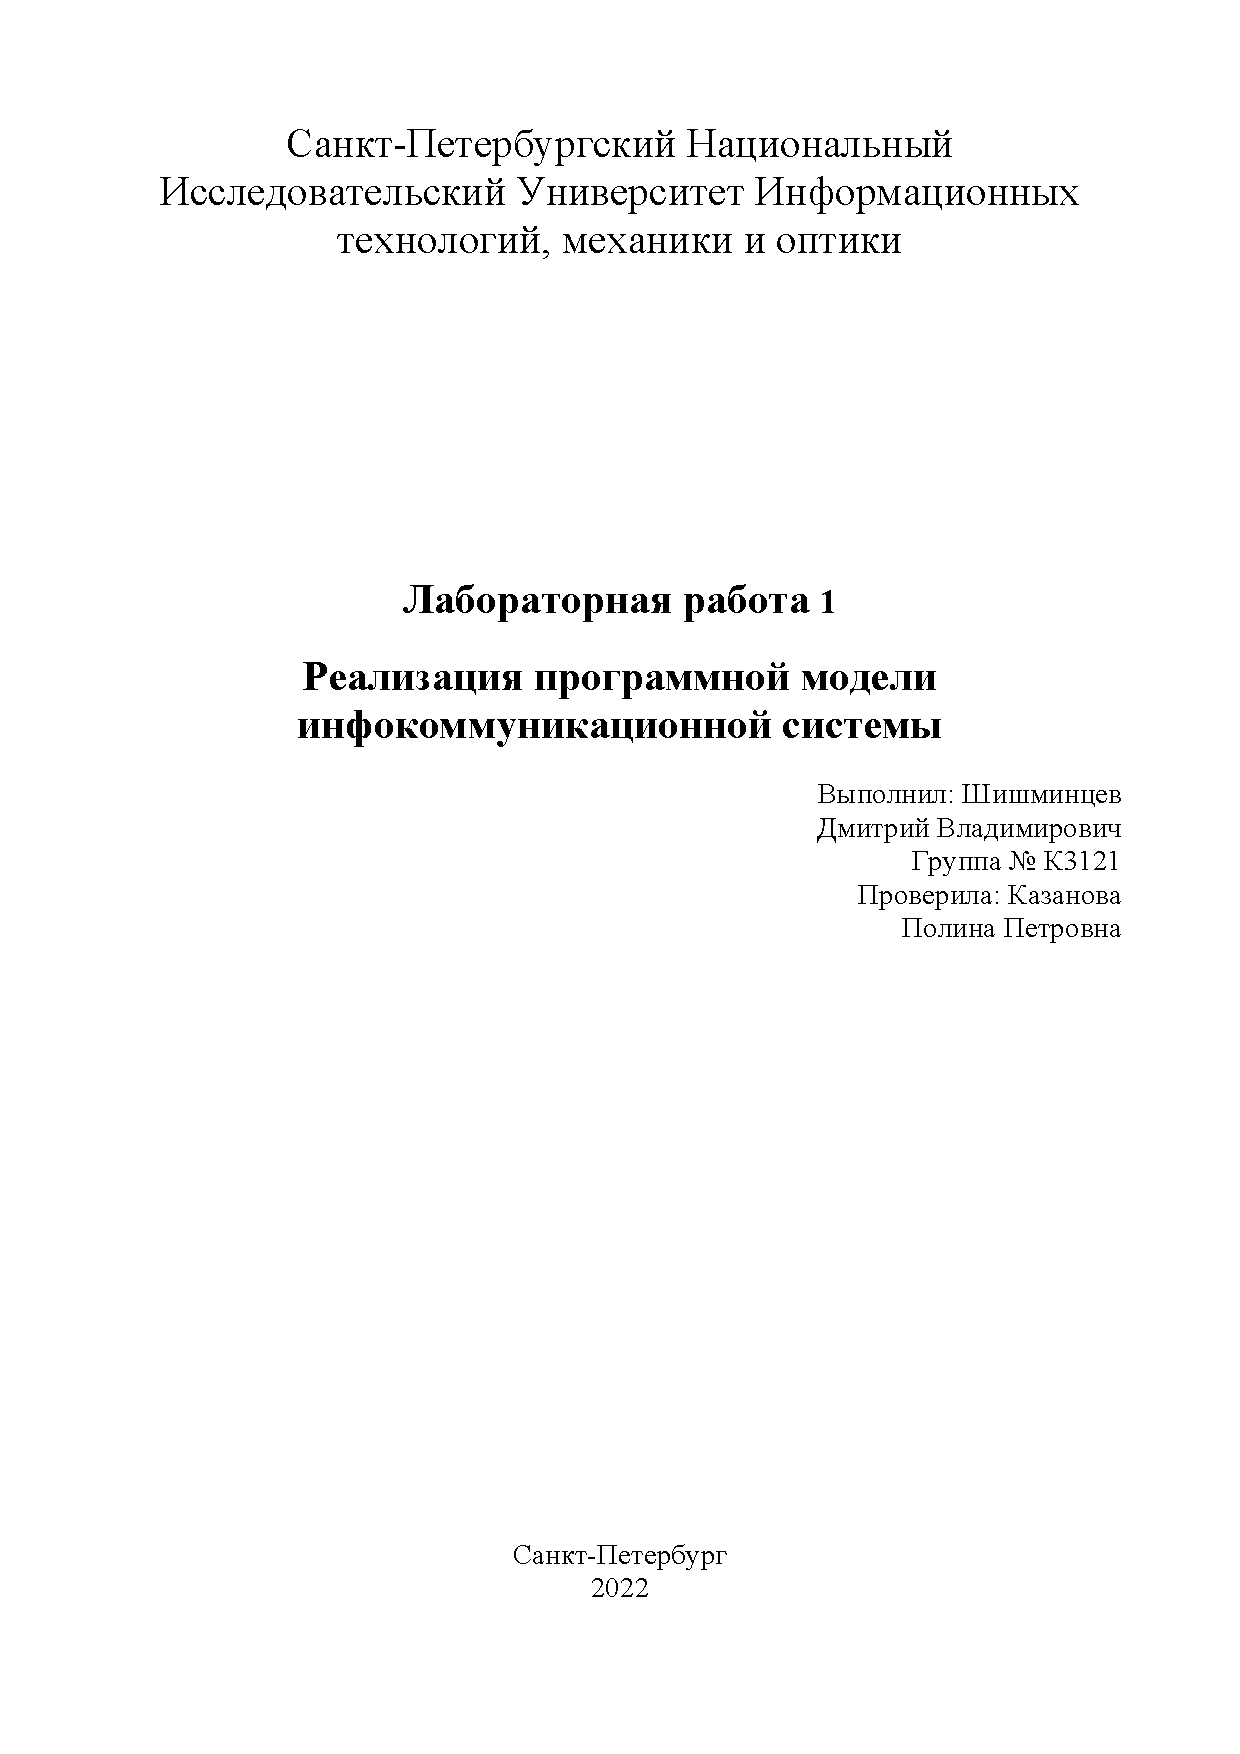
\includepdf[pages=-,pagecommand={}]{titlePage.pdf}


\pagestyle{plain} % включаем нумерацию
\tableofcontents
\intro\label{intro} 

В данной лабораторной работе была реализована система обработки данных <<Программа для контроля собственных денежных средств>>, а так же проанализирована предметная область и требования к работе.

\chapter{Анализ}
\section{Анализ предметной области}

На рынке представлено множество программного обеспечения со схожим функционалом. Их можно разделить на несколько типов: мобильные приложения банков, приложения для ручного ввода трат, приложения которые синхронизируются с банковскими приложениями. Все представленное на рынке программное обеспечение имеет следующий общий функционал: ручное/автоматическое добавление транзакций, удаление, отображение транзакций по дате, отображение транзакций по категориям, сортировка по другим параметрам. Учитывая рост спроса на потребительские товары и услуги по всему миру, область перспективной, а разработку данной программной модели - актуальной.

\section{Анализ требований}

Проанализировав предметную область, а так же задание полученное на практике по дисциплине <<Программирование>>, были выдвинуты следующие технические требования к программной модели: 
\begin{enumerate}
    \item Спроектировать базу данных SQLite3
    \item Разработать веб-сервер для статических файлов с помощью языка программирования Python и библиотеки Flask
    \item Разработать веб-сервер для обработки POST и GET запросов.
    \item Разработать веб-интерфейс для программной модели.
\end{enumerate}

\chapter{Ход работы}
\section{Проектирование базы данных SQLite3}

Для разработки модели программной системы было решено использовать систему управления базами данных SQLite3. Данная СУБД имеет такие преимущества, как: высокая скорость, кроссплатформенность, надежность, а так же не нуждается в конфигурации. 

Для хранения транзакций была спроектирована следуящая модель базы данных. Модель включает в себя одну таблицу <<transactions>>, записи в которой имеют такие свойства, как: 
\begin{enumerate}
    \item tr-id - id транзакции, так же является primary key для таблицы (integer)
    \item name - название транзакции (string)
    \item cost - стоимость транзакции (integer)
    \item date - дата транзакции. Для хранения дат было приято решение хранить их в формате unix-time. (integer)
    \item category - категория транзакции (string)
\end{enumerate}

Ниже демонстрируется схема базы данных (Рисунок \ref{fig:d1}). 

\begin{figure}[h]   
    \centering
    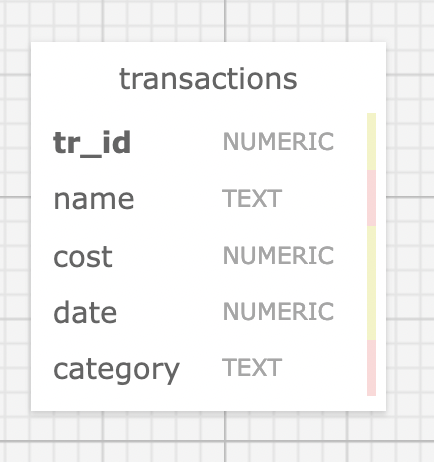
\includegraphics[width=0.5\linewidth]{db.png}
    \caption{ Схема базы данных }
    \label{fig:d1}
\end{figure}

\section{Разраотка веб-сервера для статических файлов}

Для реализации модели программной системы используется высокоуровневый язык программирования Python. Для ускорения процесса разработки было принято использовать фреймворк для создания веб-приложений Flask.

\conclusions
1


\newpage
\begin{thebibliography}{99}
	\bibitem{bib1} 	\label{bib:bib1} 1
\end{thebibliography}

\end{document}
